\documentclass{article}
\usepackage[pdftex]{graphicx}

\title{Pythorient - a lightweight script to add some functionality in the analysis of EBSD data}

\author{J\"orn Leuthold}


\date{\today}
% Hint: \title{what ever}, \author{who care} and \date{when ever} could stand 
% before or after the \begin{document} command 
% BUT the \maketitle command MUST come AFTER the \begin{document} command! 
\begin{document}

\maketitle


\begin{abstract}
Pythorient was developed for the identification of CSL $\Sigma$ triple junction configurations, which is particularly useful in terms of grain boundary engineering.  


\end{abstract}

\section{Introduction}
\begin{figure}[ht]
\centering
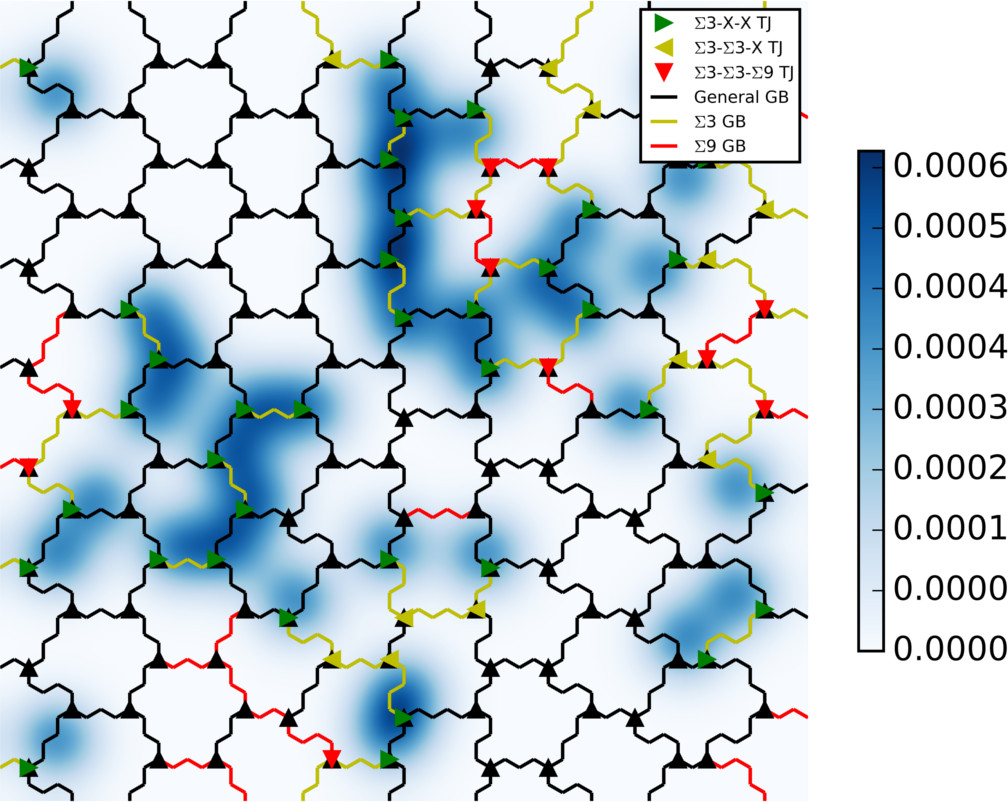
\includegraphics[width=\linewidth]{figs/Generated_OIM}
\caption{Legend (350 words max). Example legend text.}
\label{fig:generated}
\end{figure}

\begin{figure}[ht]
\centering
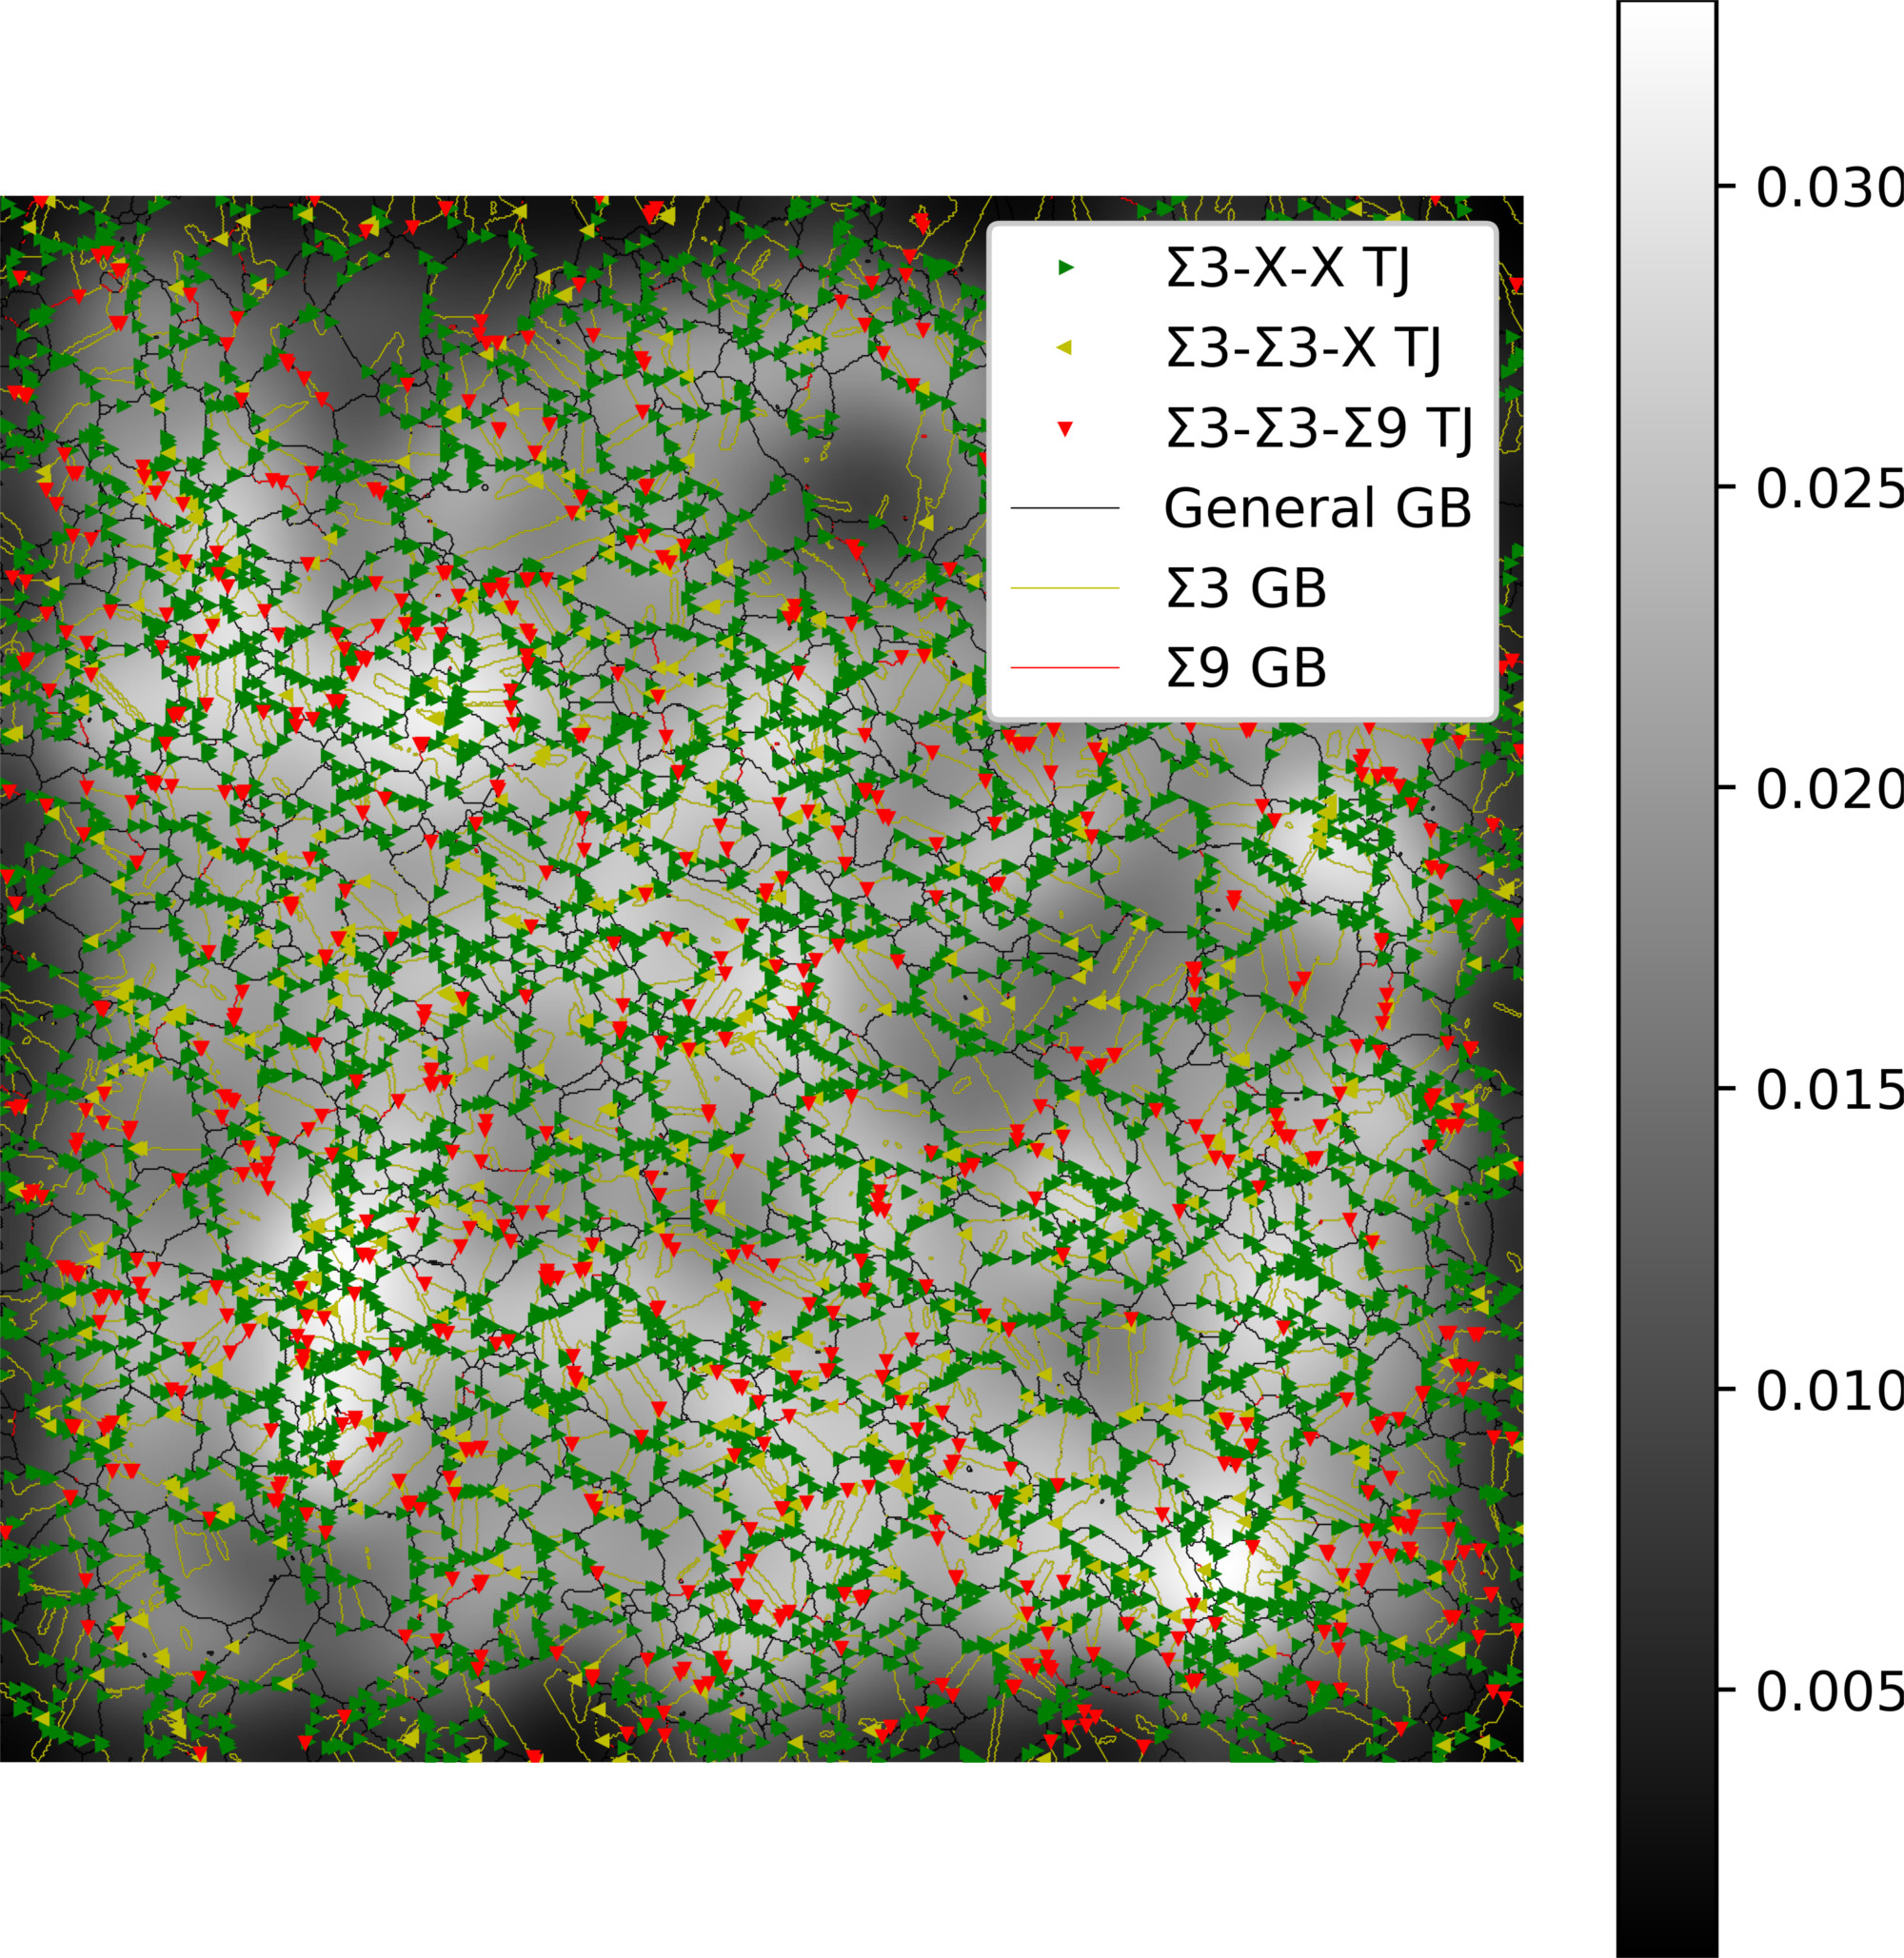
\includegraphics[width=\linewidth]{figs/Cu_TJ_analysis}
\caption{Legend (350 words max). Example legend text.}
\label{fig:stream}
\end{figure}
\end{document}

